\chapter{Projekt konceptualny}
\label{cha:konceptualny}

\section{Sformułowanie zadania projektowego}
\label{sec:sforzadproj}

Temat niniejszego projektu poświęcony jest zagadnieniu prowadzenia sesji role-playing games zwanych także grami wyobraźni. Naszym celem jest projekt oraz implementacja serwisu internetowego skupiającego miłośników tego typu rozrywki w jednym miejscu. Miałby on m.in. pośredniczyć w organizowaniu sesji zarówno w formie spotkań on-line jak i off-line, pomagać graczom w tworzeniu kart postaci czy też pozwalać przechowywać scenariusze oraz inne dane dotyczące sesji. Dodatkowo miałby on do pewnego stopnia charakter portalu społecznościowego - pozwalałby użytkownikom dzielić się scenariuszami, postaciami, oceniać osoby prowadzące sesje oraz biorące w nich udział itp.

%%%%%%%%%%%%%%%%%%%%%%%%%%%%%%%%%%%%%%%%

\section{Analiza stanu wyjściowego}
\label{sec:stanwyjsciowy}

Poszukiwania przeprowadzone w Internecie nie dały prawie żadnych rezultatów. Nie istnieje żaden serwis, który obejmowałby tematykę sesji RPG w tak szerokim zakresie. Istnieją jednak pewne rozwiązania cząstkowe. Odnaleźliśmy fora dyskusyjne, gdzie ludzie starają się prowadzić sesje, pisząc posty w wyznaczonej kolejności bądź też przykłady oprogramowania typu stand-alone, które pozwala tworzyć karty postaci i dedykowane jest pojedynczym systemom, np. Dungeons \& Dragons. Ponadto pewną ciekawostką jest istnienie interaktywnych dokumentów PDF z kartami postaci.

%%%%%%%%%%%%%%%%%%%%%%%%%%%%%%%%%%%%%%%%

\section{Analiza wymagań użytkownika}
\label{sec:wymagania}

Poniżej znajduje się wstępny zakres funkcjonalności, przy czym priorytet każdego punktu został określony wg metody MoSCoW.

\renewcommand{\labelitemi}{$\bullet$}
\renewcommand{\labelitemii}{$\circ$}

\begin{itemize}
\item rejestracja użytkowników (M)
	\begin{itemize}
	\item aktywacja konta po kliknięciu w link z powiadomienia na mailu (C)
	\item ręczna aktywacja konta przez administrację (C)
	\end{itemize}
\item logowanie użytkowników (M)
\item resetowanie haseł użytkowników (wiadomość z wygenerowanym losowym hasłem na mail) (M)
\item banowanie użytkowników przez administrację (S)
\item wspomaganie organizowania sesji RPG (M)
	\begin{itemize}
	\item tworzenie / edycja / usuwanie / odpowiadanie na ogłoszenia (M)
		\begin{itemize}
		\item „poszukuję graczy” (M)
		\item „poszukuję mistrza gry” (M)
		\end{itemize}
	\item lista ogłoszeń (M)
	\item filtrowanie listy ogłoszeń (M)
	\end{itemize}
\item sesje RPG jako spotkania on-line (M)
	\begin{itemize}
	\item czat (M)
		\begin{itemize}
		\item okno sesji (M)
			\begin{itemize}
			\item lista uczestników (M)
			\item informacje o sesji (M)
			\item informacje o uczestnikach (M)
			\item rzuty kostkami wielościennymi (M)
			\end{itemize}
		\item możliwość rysowania w trakcie sesji (C)
		\end{itemize}
	\end{itemize}
\item tworzenie kart postaci dla wybranego systemu(-ów) (S)
\item charakter społecznościowy (S)
	\begin{itemize}
	\item przesyłanie prywatnych wiadomości pomiędzy użytkownikami (S)
	\item ocenianie mistrzów gry (S)
	\item ocenianie graczy (S)
	\item ustawienia prywatności / opcje udostępniania (S)
	\end{itemize}
\item baza systemów RPG (C)
\item eksport kart postaci oraz innych danych do wybranego formatu, np. pdf (C)
\item wersja mobilna serwisu (C)
\item generatory imion (C)
\item moduł sklepu pozwalający na zakup podręczników oraz innych akcesoriów związanych z sesjami RPG (W)
\end{itemize}

%%%%%%%%%%%%%%%%%%%%%%%%%%%%%%%%%%%%%%%%

\section{Przypadki użycia}
\label{sec:przypadki}

\renewcommand{\labelenumi}{\arabic{enumi}.} 
\renewcommand{\labelenumii}{\arabic{enumi}.\arabic{enumii}.}
\renewcommand{\labelenumiii}{\arabic{enumi}.\arabic{enumii}.\arabic{enumiii}.}

\begin{enumerate}
\item Gość:
	\begin{enumerate}
	\item Rejestracja konta,
	\item Logowanie,
	\item Przeglądanie ogłoszeń,
	\item Przeglądanie profili użytkowników,
	\item Przeglądanie systemów RPG,
	\item Resetowanie hasła.
	\end{enumerate}
\item Użytkownik:
	\begin{enumerate}
	\item Zarządzanie kontem,
	\item Tworzenie / Edycja / Usuwanie ogłoszeń,
	\item Akceptowanie zgłoszeń graczy / MG,
	\item Odpowiadanie na ogłoszenia,
	\item Uczestniczenie w sesji on-line,
	\item Tworzenie / Edycja / Usuwanie scenariuszy,
	\item Tworzenie / Edycja / Usuwanie kart postaci,
	\item Ocenianie użytkowników,
	\item Przesyłanie prywatnych wiadomości.
	\end{enumerate}
\item Moderator:
	\begin{enumerate}
	\item Edycja / Usuwanie ocen i komentarzy,
	\item Dodawanie / Edycja / Usuwanie systemów RPG.
	\end{enumerate}
\item Administrator:
	\begin{enumerate}
	\item Zarządzanie użytkownikami:
		\begin{enumerate}
		\item Ręczna aktywacja konta użytkownika,
		\item Banowanie kont.
		\end{enumerate}
	\end{enumerate}
\end{enumerate}


%%%%%%%%%%%%%%%%%%%%%%%%%%%%%%%%%%%%%%%%

\clearpage
\section{Wybrane scenariusze użycia}
\label{sec:scenariusze}

Lorem ipsum.

%%%%%%%%%%%%%%%%%%%%%%%%%%%%%%%%%%%%%%%%

\section{Identyfikacja funkcji}
\label{sec:idfun}

Główną funkcją realizowaną przez bazę danych jest przechowywanie informacji o:
	\begin{itemize}
	\item kontach użytkowników wraz z dodatkowymi informacjami (ustawieniami, ocenami, wiadomościami prywatnymi),
	\item ogłoszeniach dotyczących sesji wraz z powiązaniami do kont,
	\item postaciach graczy wraz z powiązaniami do kont,
	\item scenariuszach wraz z powiązaniami do kont,
	\item systemach RPG.
	\end{itemize}

%%%%%%%%%%%%%%%%%%%%%%%%%%%%%%%%%%%%%%%%

\clearpage

\section{FHD - diagram hierarchii funkcji}
\label{sec:FHD}

\setlength{\DTbaselineskip}{15pt}
\dirtree{%
.1 Sesje RPG.
	.2 Konta użytkowników.
		.3 Utworzenie konta.
			.4 Rejestracja.
			.4 Aktywacja.
		.3 Logowanie.
		.3 Ustawienia konta.
			.4 Ustawienia prywatności.
			.4 Ustawienia powiadomień.
			.4 Ustawienia danych w profilu.
			.4 Zmiana hasła.
		.3 Resetowanie hasła.
	.2 Ogłoszenia. 
		.3 Tworzenie ogłoszeń.
		.3 Przeglądanie ogłoszeń.
			.4 Filtrowanie ogłoszeń.
			.4 Aplikowanie do sesji.
		.3 Zarządzanie ogłoszeniami.
			.4 Edycja / Usuwanie ogłoszeń.
			.4 Akceptacja graczy.
			.4 Udział w sesji.
	.2 Scenariusze.
		.3 Tworzenie / Edycja / Usuwanie scenariuszy.
	.2 Karty postaci.
		.3 Tworzenie / Edycja / Usuwanie kart postaci.
	.2 Społeczność. 
		.3 Ocenianie użytkowników.
			.4 Wystawianie / Edycja oceny z komentarzem.
		.3 Przesyłanie prywatnych wiadomości.
	.2 Systemy RPG.
		.3 Przeglądanie bazy systemów RPG.
	.2 Administracja.
		.3 Zarządzanie użytkownikami.
			.4 Ręczna aktywacja kont.
			.4 Banowanie kont.
		.3 Zarządzanie systemami RPG.
			.4 Dodawanie / Edycja / Usuwanie systemów.
		.3 Moderacja.
			.4 Edycja / Usuwanie ocen i komentarzy.
}

%%%%%%%%%%%%%%%%%%%%%%%%%%%%%%%%%%%%%%%%

\clearpage 
\section{DFD - diagramy przepływu danych}
\label{sec:DFD}

Lorem ipsum.

%%%%%%%%%%%%%%%%%%%%%%%%%%%%%%%%%%%%%%%%

\section{Encje i atrybuty}
\label{sec:encje}

\begin{enumerate}
\item Użytkownik:
	\begin{itemize}
	\item login (e-mail),
	\item hash MD5 hasła,
	\item status konta,
	\item poziom uprawnień,
	\item ustawienia,
	\item dane użytkownika.
	\end{itemize}
\item Ogłoszenie:
	\begin{itemize}
	\item twórca,
	\item system,
	\item czas utworzenia
	\item data,
	\item typ,
	\item miejsce,
	\item uczestnicy wraz z rolami.
	\end{itemize}
\item System RPG:
	\begin{itemize}
	\item nazwa,
	\item opis,
	\item gatunek,
	\item projektant,
	\item wydawca,
	\item rok,
	\item DTD karty postaci.
	\end{itemize}
\item Karta postaci:
	\begin{itemize}
	\item autor,
	\item system,
	\item XML.
	\end{itemize}
\item Scenariusz:
	\begin{itemize}
	\item autor,
	\item system,
	\item typ,
	\item sugerowana ilość graczy,
	\item treść.
	\end{itemize}
\item Wiadomość:
	\begin{itemize}
	\item nadawca,
	\item adresat,
	\item timestamp,
	\item temat,
	\item treść,
	\item czy przeczytana.
	\end{itemize}
\item Komentarz:
	\begin{itemize}
	\item komentujący,
	\item komentowany,
	\item ocena,
	\item komentarz,
	\item timestamp.
	\end{itemize}
\end{enumerate}

%%%%%%%%%%%%%%%%%%%%%%%%%%%%%%%%%%%%%%%%

\clearpage
\section{ERD - diagram związków encji}
\label{sec:ERD}

\begin{figure}[h!]
\begin{center}
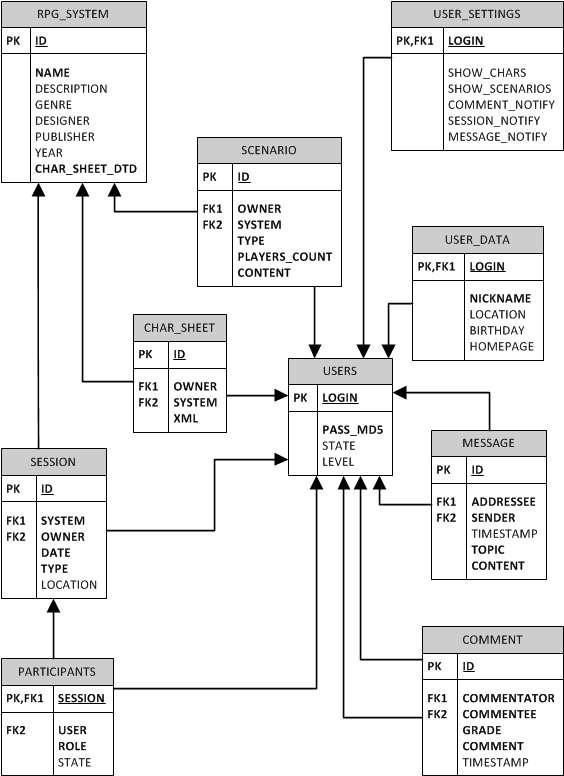
\includegraphics[scale=1]{./img/ERD.png}
\caption[Diagram związków encji]{Diagram związków encji}
\label{fig:ERD}
\end{center}
\end{figure}

%%%%%%%%%%%%%%%%%%%%%%%%%%%%%%%%%%%%%%%%

\clearpage
\section{STD - diagramy przejść pomiędzy stanami}
\label{sec:STD}

Lorem ipsum.